\documentclass[fleqn]{beamer}

\usepackage{amsmath}
\usepackage{animate}
\usepackage{amsfonts}
\usepackage[mathscr]{eucal}
\usepackage{subcaption}
\usepackage{wrapfig}
\usepackage{graphicx}

\usepackage{fancyhdr}
\usepackage{pstricks}
\usepackage{pst-func}
\usepackage{pst-plot}
\usepackage[utf8x]{inputenc}
\usepackage[spanish]{babel}


\setbeamertemplate{navigation symbols}{}
\definecolor{UniBlue}{RGB}{83,121,170}
\setbeamercolor{frametitle}{fg=black,bg=white}
\setbeamercolor{title}{fg=black,bg=yellow!85!orange}
%\setbeamercolor{title}{fg=red,bg=yellow!90!blue}
\usetheme{Madrid}

\beamersetuncovermixins{\opaqueness<1>{25}}{\opaqueness<2->{15}}
\begin{document}

\title{CGeIHC}
\author{Reynaldo Martell}
\date{\today} 

\begin{frame}
\titlepage
\end{frame}

\begin{frame}\frametitle{\rule{0mm}{10mm}\rule{5mm}{0mm} Computación Gráfica. }
Computación grafica es la representación y
manipulación de información de manera visual
mediante el uso de computadoras.
%\begin{figure}[H]
%	\centering
%	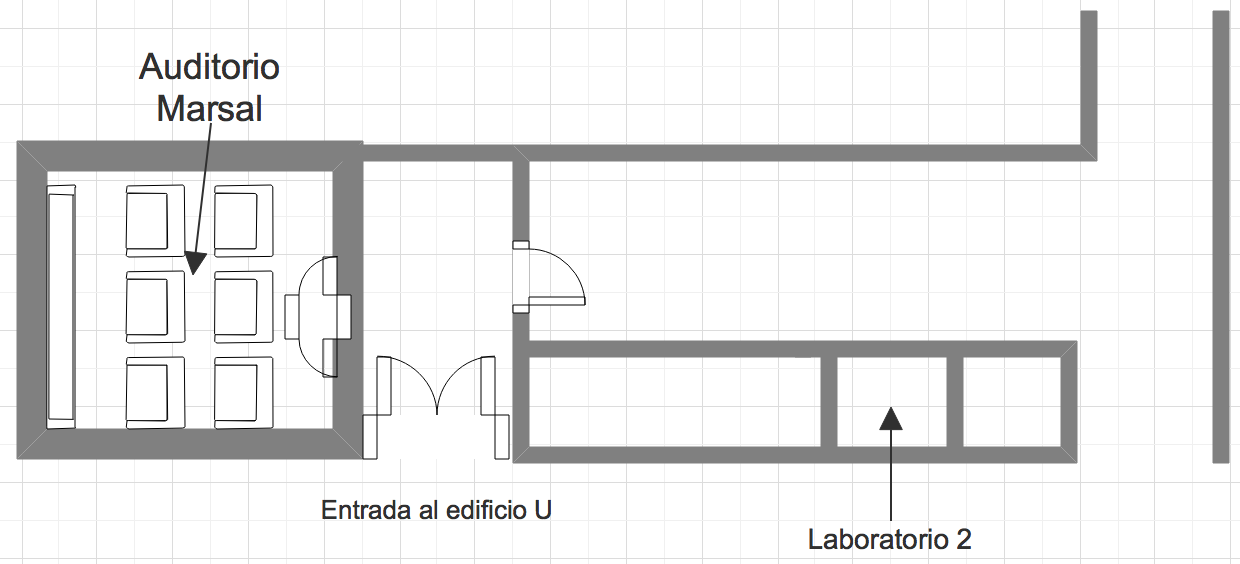
\includegraphics[width=1.0\textwidth]{images/mapa.png}
%	\label{mapa}
%\end{figure}
\end{frame}

\begin{frame}\frametitle{\rule{0mm}{10mm}\rule{5mm}{0mm} Computación Gráfica. }
\begin{itemize}
	\item Despliegue de información.
	\begin{itemize}
		\item Aplicaciones médicas (visualización científica).
		\begin{itemize}
			\item Ultrasonidos.
			\item Tomografías.
			\item Generación de datos 3D que a los que se la aplican algoritmos de
manipulación para proporcionar información útil.
Diseño (CAD). Proporcionan una interfaz interactiva.
		\end{itemize}
	\end{itemize}
	\item Diseño (CAD). Proporcionan una interfaz interactiva.
	\begin{itemize}
		\item Arquitectura.
		\item Diseño de partes mecánicas.
		\item Circuitos VLSI.
	\end{itemize}
	\item Simulación y animación.
	\begin{itemize}
		\item Simuladores de vuelo.
		\item Animación.
		\item Captura de movimiento.
	\end{itemize}
	\item Interfaces de usuario (Interacción hombre computadoras).
\end{itemize}
\end{frame}

\begin{frame}\frametitle{\rule{0mm}{10mm}\rule{5mm}{0mm} Sistema Gráfico. }
Sistema grafico: es un sistema de computadora que debe tener todos los
siguientes componentes:
\begin{itemize}
	\item Dispositivos de entrada.
	\item CPU.
	\item GPU.
	\item Memoria.
	\item Framebuffer.
	\item Dispositivos de salida.
	
\begin{figure}[H]
	\centering
	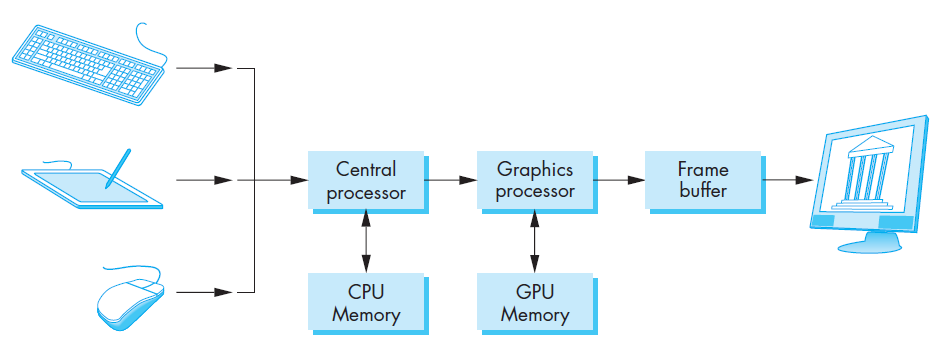
\includegraphics[width=0.7\textwidth]{images/SistemaGrafico.png}
	\label{mapa}
\end{figure}
\end{itemize}
\end{frame}

\begin{frame}\frametitle{\rule{0mm}{10mm}\rule{5mm}{0mm} Pixels and the Framebuffer. }
\begin{itemize}
	\item Todos los sistemas gráficos utilizan rasterización.
	\item Rasterización se refiera a la conversión de elementos geométricos al color del pixel y posición en el framebuffer.
	\item Las imágenes que vemos en los dispositivos de salida son arreglos de pixeles.
	\item Los pixeles son guardados juntos en una parte de memoria llamada framebuffer.	
	
\begin{figure}[htb]
	\centering
	\begin{tabular}{@{}cccc@{}}
		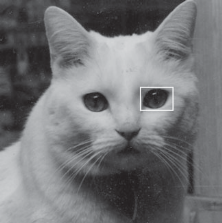
\includegraphics[width=.23\textwidth]{images/FrameBuffer1.png} &
    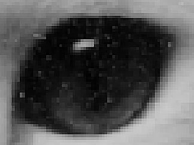
\includegraphics[width=.23\textwidth]{images/FrameBuffer2.png} &
	\end{tabular}
	\label{mapa}
\end{figure}
\end{itemize}
\end{frame}

%%%%%% Hardware and software
\begin{frame}\frametitle{\rule{0mm}{10mm}\rule{5mm}{0mm} Hardware y Software - Cronología. }
1946 - Primera computadora de propósito general ENIAC
\begin{figure}[H]
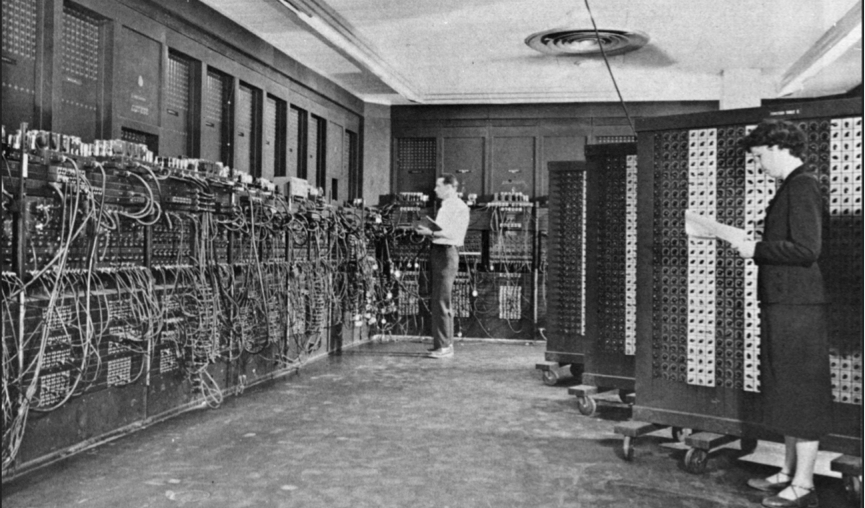
\includegraphics[width=.8\textwidth]{images/ENIAC.png}
\end{figure}
\end{frame}

\begin{frame}\frametitle{\rule{0mm}{10mm}\rule{5mm}{0mm} Hardware y Software - Cronología. }
1950 – Tubo de rayos catódicos.
\begin{figure}[H]
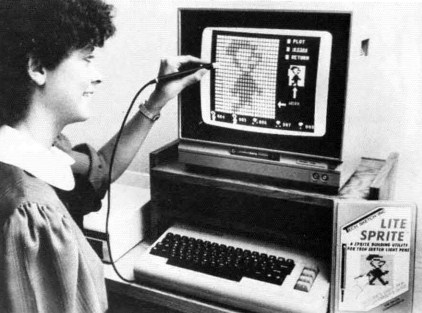
\includegraphics[width=.6\textwidth]{images/TuboRayos.png}
\end{figure}
\end{frame}

\begin{frame}\frametitle{\rule{0mm}{10mm}\rule{5mm}{0mm} Hardware y Software - Cronología. }
1952 – OXO - EDSAC (Electronic Delay Storage Automatic Calculator)
\begin{figure}[H]
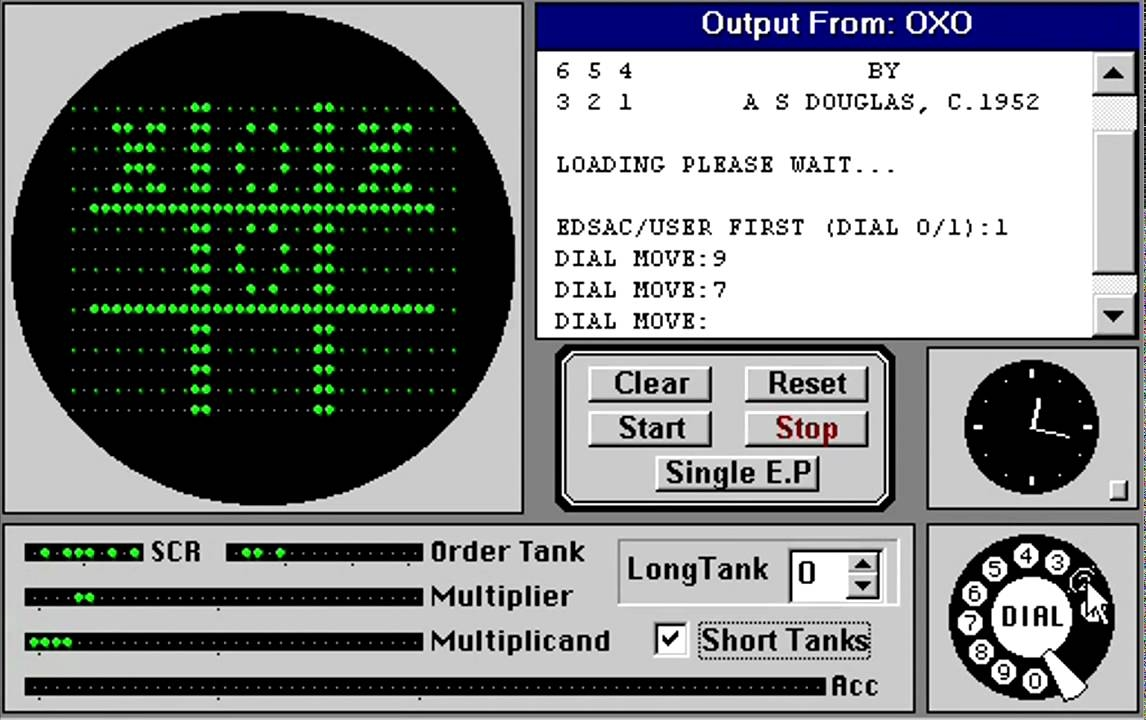
\includegraphics[width=.8\textwidth]{images/OXO.png}
\end{figure}
\end{frame}

\begin{frame}\frametitle{\rule{0mm}{10mm}\rule{5mm}{0mm} Hardware y Software - Cronología. }
1962 - Spacewar
\begin{figure}[htb]
	\centering
	\begin{tabular}{@{}cccc@{}}
		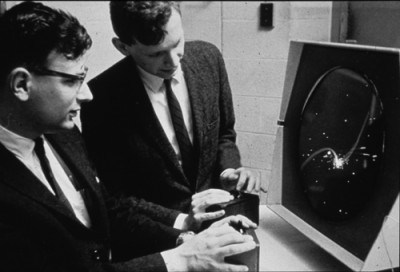
\includegraphics[width=.45\textwidth]{images/SpeaceWar1.png} &
    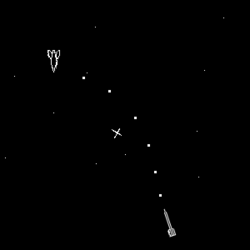
\includegraphics[width=.35\textwidth]{images/SpeaceWar2.png} &
	\end{tabular}
	\label{mapa}
\end{figure}
\end{frame}


\begin{frame}\frametitle{\rule{0mm}{10mm}\rule{5mm}{0mm} Hardware y Software - Cronología. }
1962 - Sketchpad Ivan Sutherland
\begin{figure}[H]
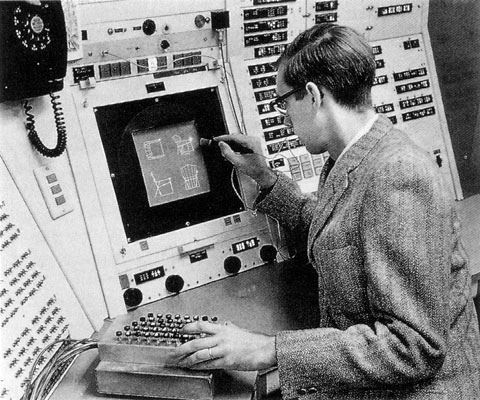
\includegraphics[width=.6\textwidth]{images/Sketchpad.png}
\end{figure}
\end{frame}

\begin{frame}\frametitle{\rule{0mm}{10mm}\rule{5mm}{0mm} Hardware y Software - Cronología. }
1966 – The Sword of Damocles, primer sistema de realidad virtual, así como desarrollo formal de las Interfaces Gráficas de Usuario.
\begin{figure}[H]
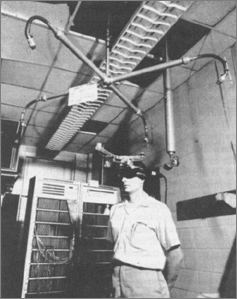
\includegraphics[width=.4\textwidth]{images/Democles.png}
\end{figure}
\end{frame}

\begin{frame}\frametitle{\rule{0mm}{10mm}\rule{5mm}{0mm} Hardware y Software - Cronología. }
1971 – Microprocesador. \\
1972 – Atari y videojuego Pong.
\begin{figure}[htb]
	\centering
	\begin{tabular}{@{}cccc@{}}
		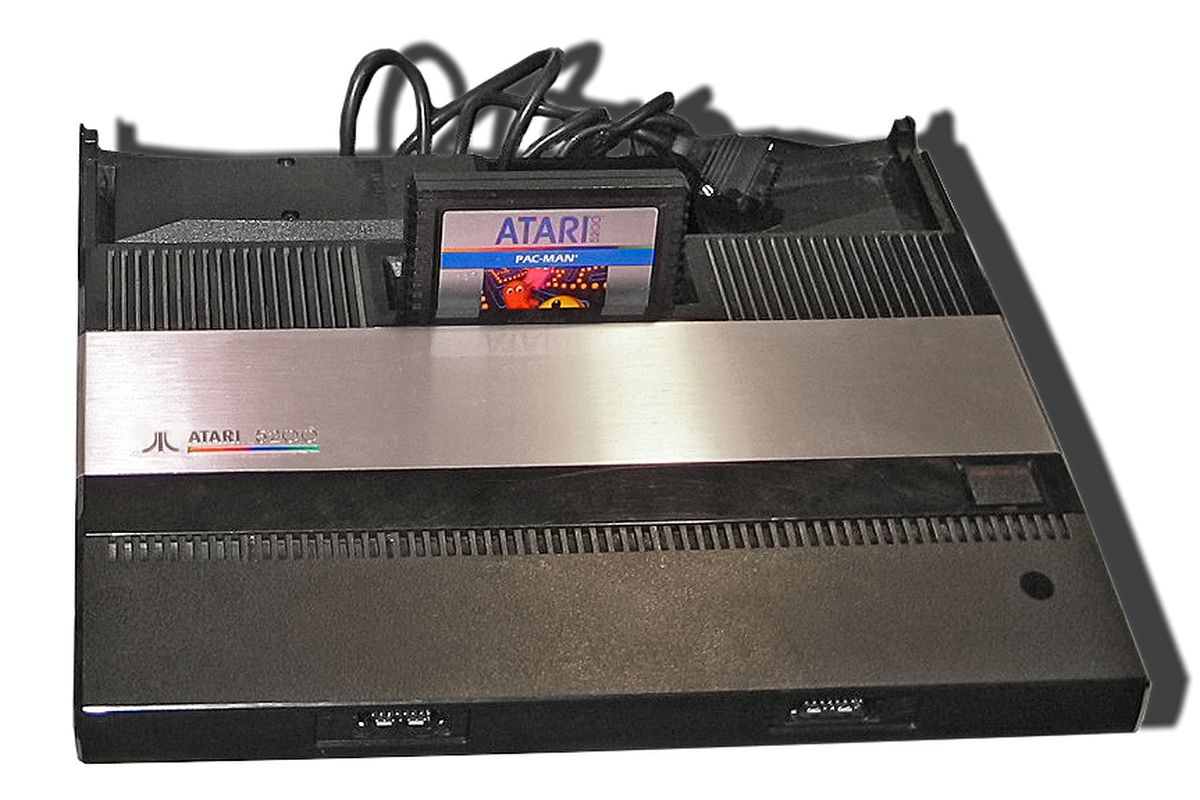
\includegraphics[width=.3\textwidth]{images/Atari1.png} &
    	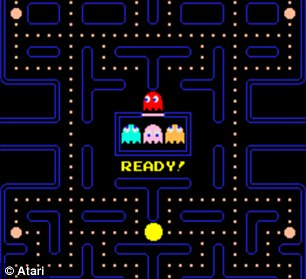
\includegraphics[width=.2\textwidth]{images/Atari2.png} &
    	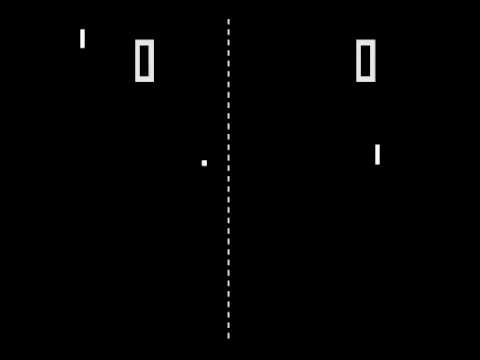
\includegraphics[width=.25\textwidth]{images/Atari3.png}
	\end{tabular}
	\label{mapa}
\end{figure}

\end{frame}

\begin{frame}\frametitle{\rule{0mm}{10mm}\rule{5mm}{0mm} Hardware y Software - Cronología. }
1980 – SIGGRAPH (Special Interested Group on Graphics). Loren Carpenter
\end{frame}

\begin{frame}\frametitle{\rule{0mm}{10mm}\rule{5mm}{0mm} Hardware y Software - Cronología. }
1992 – OpenGL.
\begin{figure}[htb]
	\centering
	\begin{tabular}{@{}cccc@{}}
		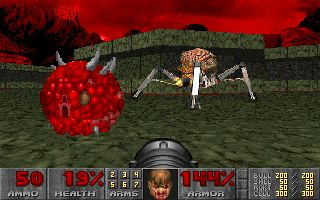
\includegraphics[width=.4\textwidth]{images/Doom.png} &
    	
\includegraphics[width=.4\textwidth]{images/OpenGL.png}
	\end{tabular}
	\label{mapa}
\end{figure}
\end{frame}

\begin{frame}\frametitle{\rule{0mm}{10mm}\rule{5mm}{0mm} Hardware y Software - Cronología. }
1994 – Primer acelerador gráfico, 3Dfx Voodoo 3D.
\begin{figure}[H]
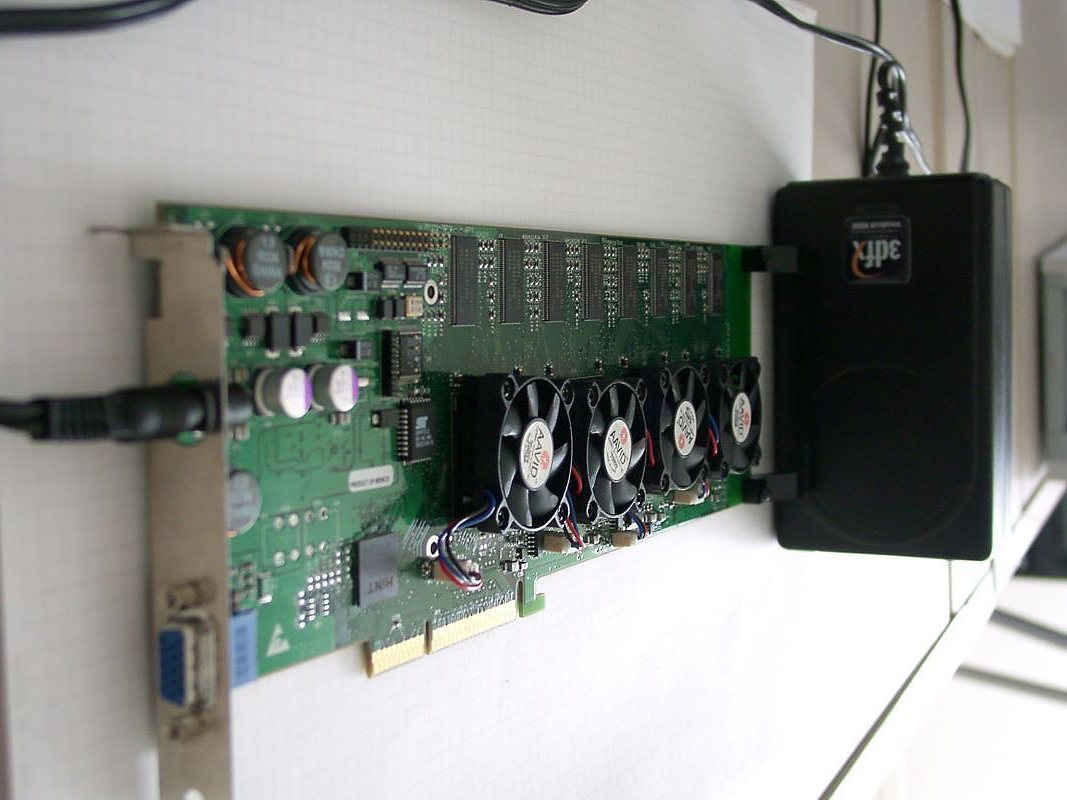
\includegraphics[width=.7\textwidth]{images/3Dfx.png}
\end{figure}
\end{frame}

\begin{frame}\frametitle{\rule{0mm}{10mm}\rule{5mm}{0mm} Hardware y Software - Cronología. }
1999 – Aparición del primer GPU (Graphics Processing Unit). 
\begin{figure}[htb]
	\centering
	\begin{tabular}{@{}cccc@{}}
		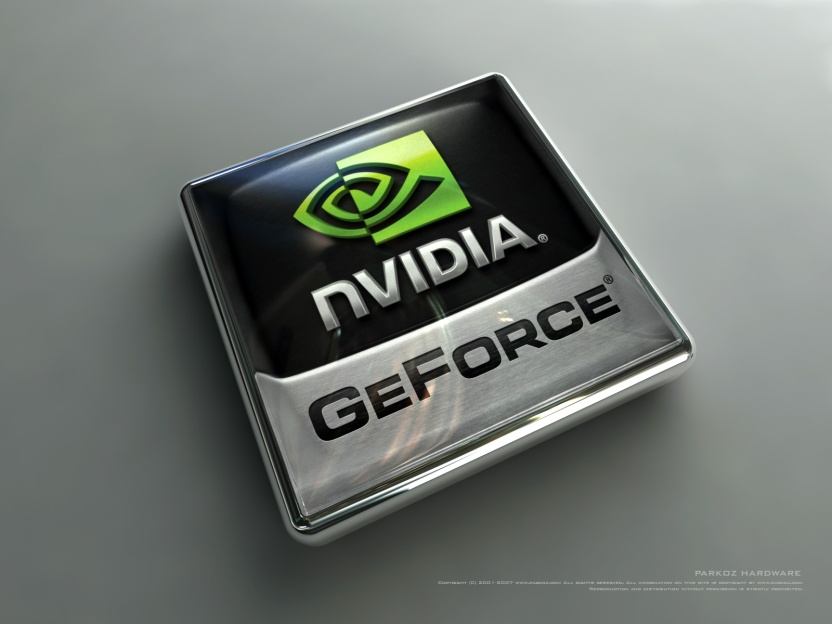
\includegraphics[width=.4\textwidth]{images/GPU1.png} &
    	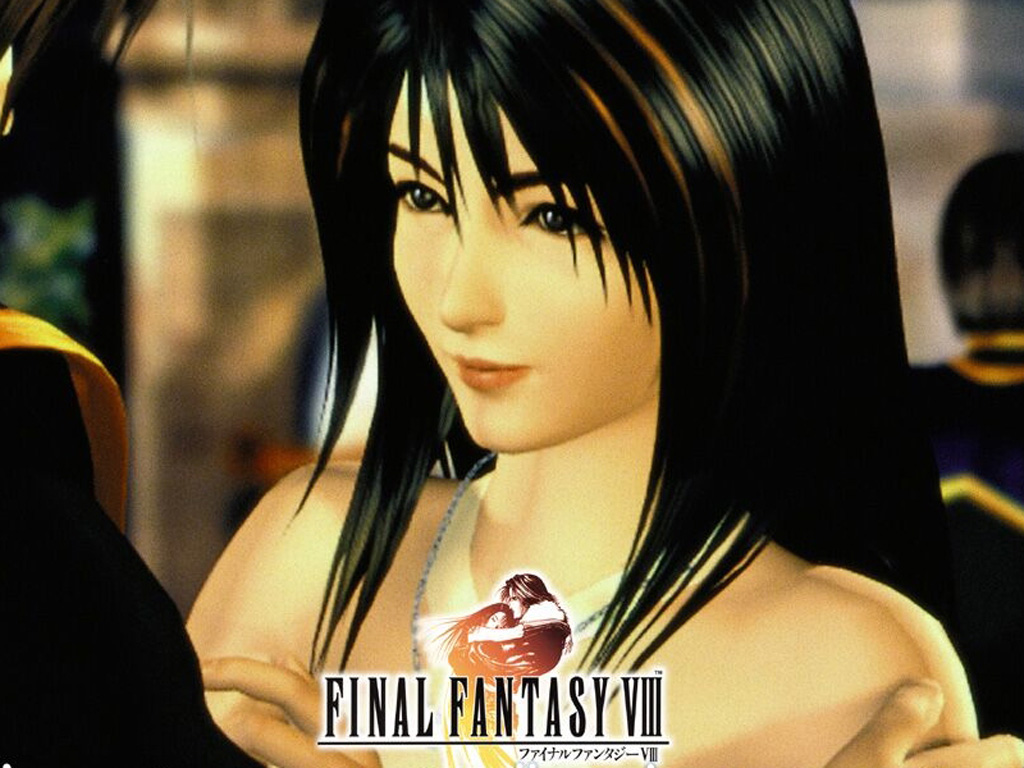
\includegraphics[width=.4\textwidth]{images/FinalFantasy.png}
	\end{tabular}
	\label{mapa}
\end{figure}
\end{frame}

\begin{frame}\frametitle{\rule{0mm}{10mm}\rule{5mm}{0mm} Hardware y Software - Cronología. }
2003 – Shaders. “Física” en aplicaciones.
\begin{figure}[H]
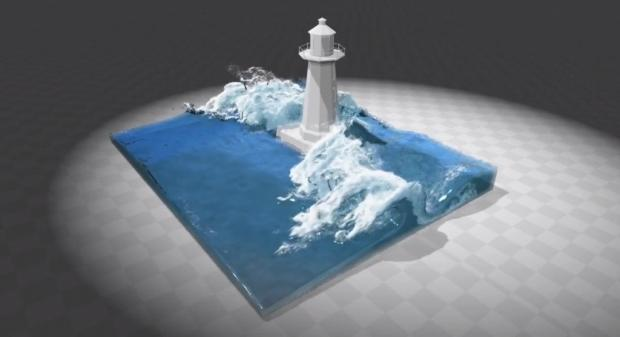
\includegraphics[width=.8\textwidth]{images/Fisica.png}
\end{figure}
\end{frame}

\begin{frame}\frametitle{\rule{0mm}{10mm}\rule{5mm}{0mm} Hardware y Software - Cronología. }
2005 – GPUs en paralelo. 
\begin{figure}[htb]
	\centering
	\begin{tabular}{@{}cccc@{}}
		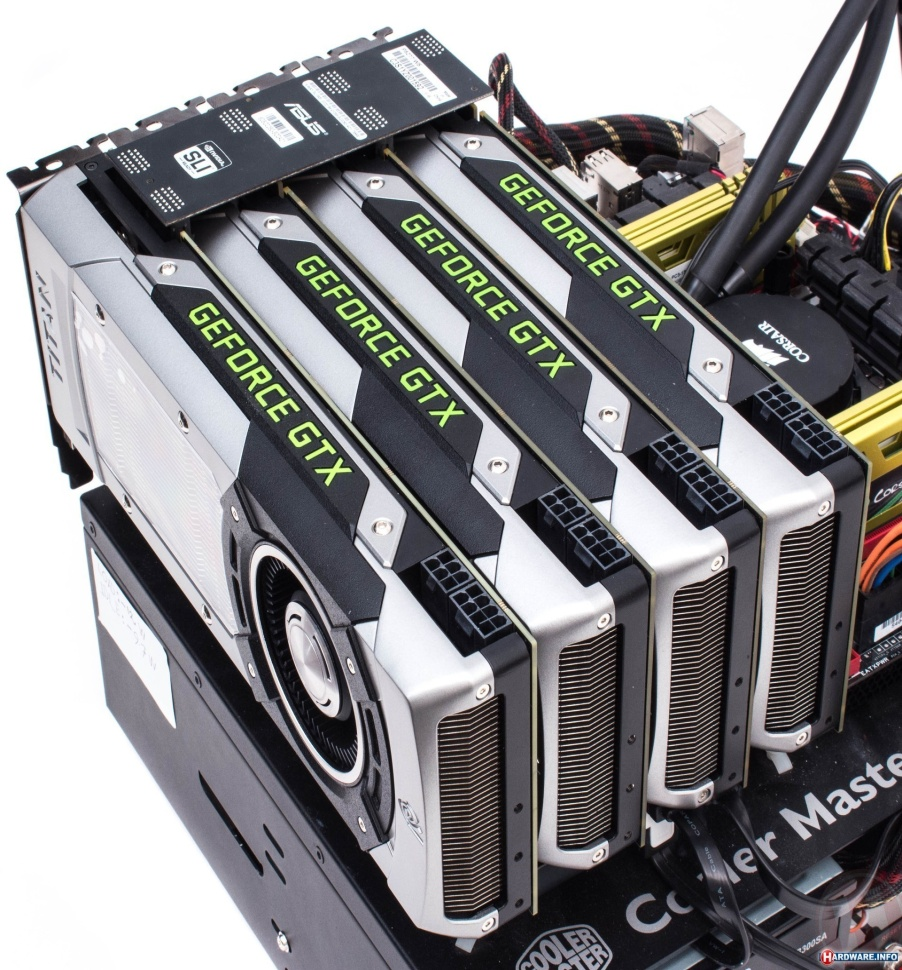
\includegraphics[width=.3\textwidth]{images/GPU2.png} &
    	
\includegraphics[width=.2\textwidth]{images/GPU3.png} &
    	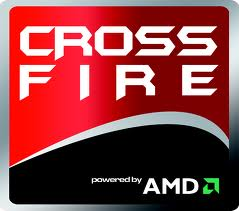
\includegraphics[width=.2\textwidth]{images/GPU4.png}
	\end{tabular}
	\label{mapa}
\end{figure}
\end{frame}

\begin{frame}\frametitle{\rule{0mm}{10mm}\rule{5mm}{0mm} Hardware y Software - Cronología. }
2010 - Dispositivos de interacción.
\begin{figure}[H]
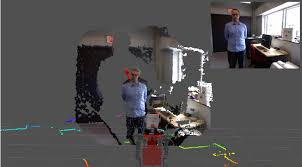
\includegraphics[width=.8\textwidth]{images/Kinect.png}
\end{figure}
\end{frame}

\begin{frame}\frametitle{\rule{0mm}{10mm}\rule{5mm}{0mm} Hardware y Software - Cronología. }
2015 – Realidad Virtual
\begin{figure}[H]
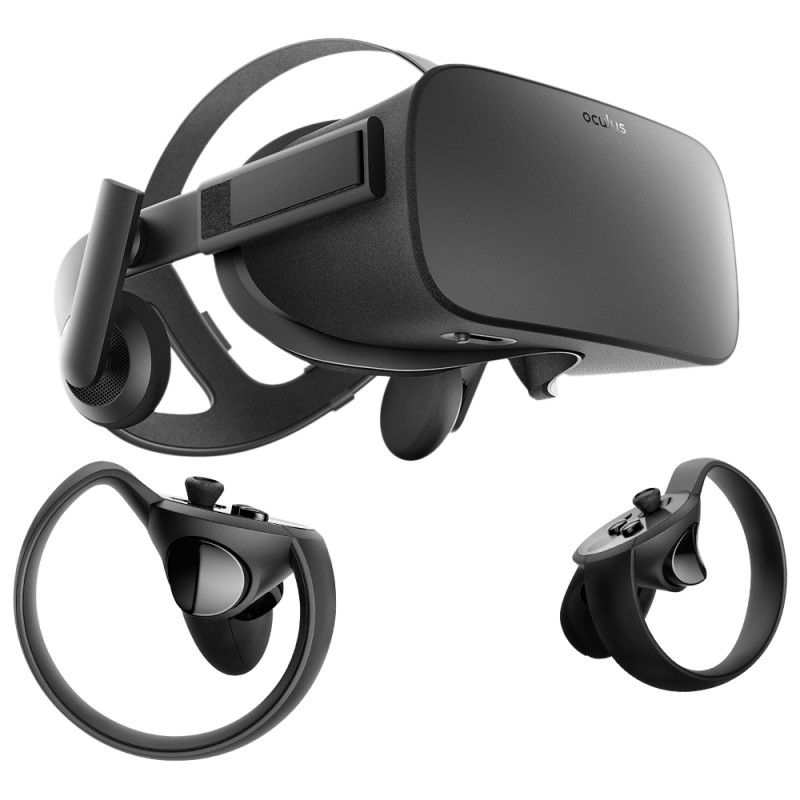
\includegraphics[width=.6\textwidth]{images/Oculus.png}
\end{figure}
\end{frame}

\begin{frame}\frametitle{\rule{0mm}{10mm}\rule{5mm}{0mm} Hardware y Software - GPU. }
\begin{figure}[H]
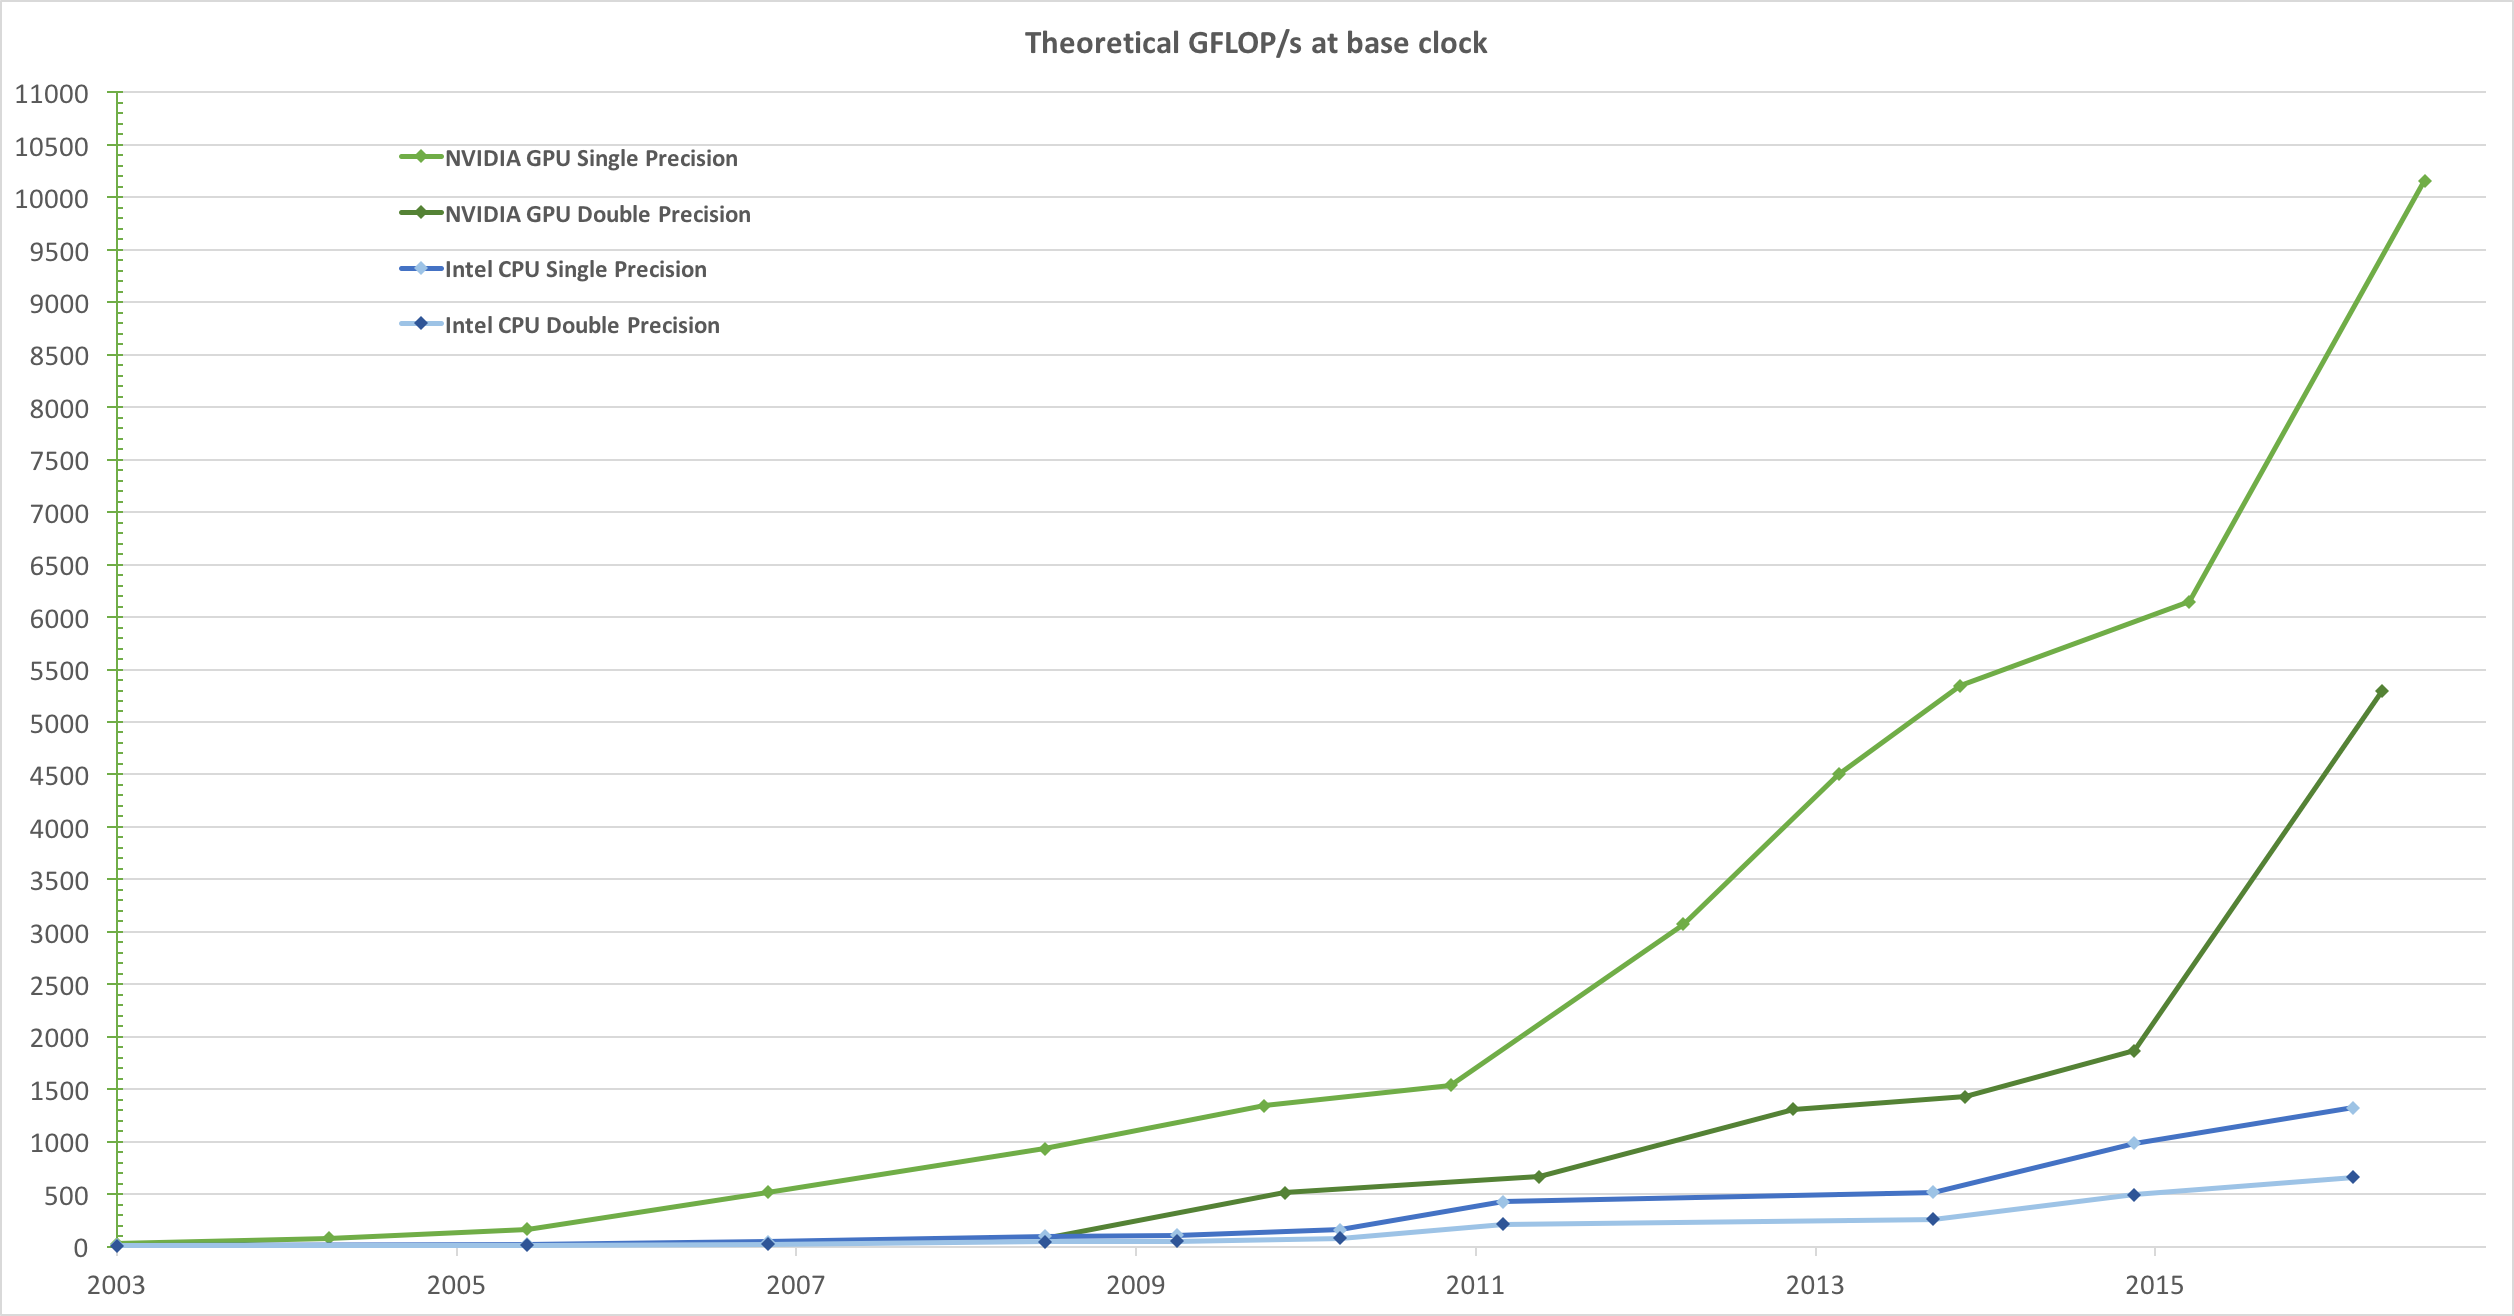
\includegraphics[width=1.0\textwidth]{images/GPU5.png}
\end{figure}
\end{frame}

\begin{frame}\frametitle{\rule{0mm}{10mm}\rule{5mm}{0mm} Ancho de banda de una CPU y GPU }
\begin{figure}[H]
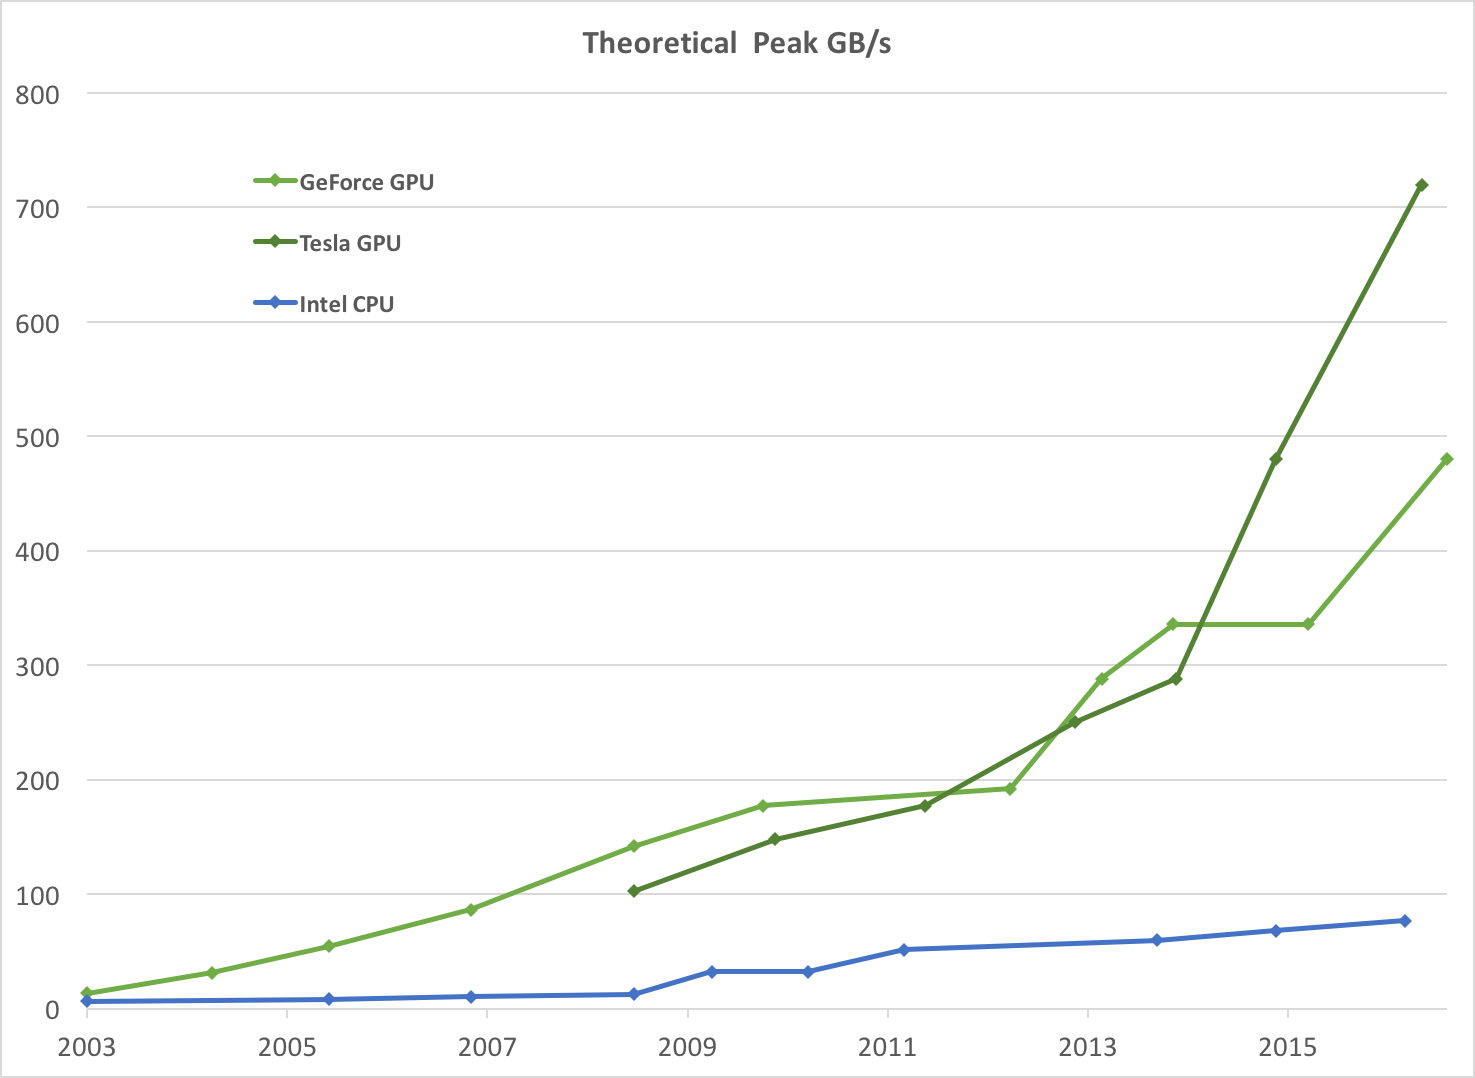
\includegraphics[width=0.8\textwidth]{images/GPU7.png}
\end{figure}
\end{frame}

\begin{frame}\frametitle{\rule{0mm}{10mm}\rule{5mm}{0mm} Hardware y Software - GPU. }
\begin{itemize}
	\item La razón detrás de la discrepancia en las capacidades de procesamiento de punto flotante entre la 	CPU y la GPU es que la GPU es especializada para computo masivo.
	\item  El mismo programa puede usar el mismo programa para procesarlos en paralelo.
	\item En renderizado 3D, un gran conjunto de pixeles y vértices son mapeados en hilos paralelos.
\end{itemize}
\begin{figure}[H]
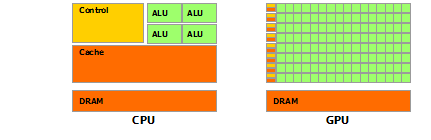
\includegraphics[width=.8\textwidth]{images/GPU8.png}
\end{figure}
\end{frame}

\begin{frame}\frametitle{\rule{0mm}{10mm}\rule{5mm}{0mm} Hardware y Software - GPU. }
De igual forma en imágenes, aplicaciones de procesamiento de medios tales como post procesamiento de imágenes ya renderizadas, codificación y decodificación de video, escalamiento de imágenes, visión estéreo y reconocimiento de patrones. 
\begin{figure}[H]
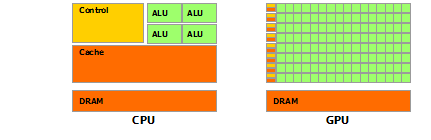
\includegraphics[width=.8\textwidth]{images/GPU8.png}
\end{figure}
\end{frame}

\begin{frame}\frametitle{\rule{0mm}{10mm}\rule{5mm}{0mm} Ancho de banda de una CPU y GPU }
\begin{figure}[H]
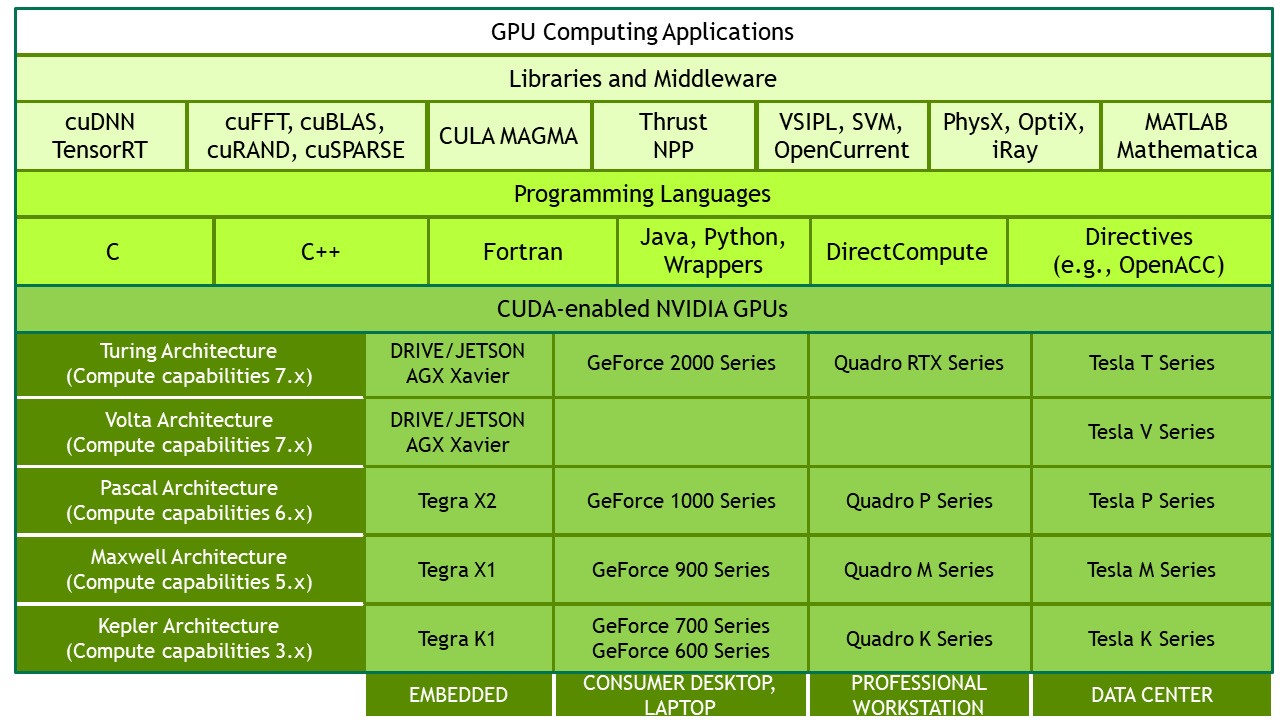
\includegraphics[width=1.0\textwidth]{images/gpu-computing-applications.png}
\end{figure}
\end{frame}

\end{document}

